\documentclass[11pt]{article}
\usepackage{amsmath, amssymb, amscd, amsthm, amsfonts}
\usepackage{graphicx}
\usepackage{hyperref}
\usepackage{commath}
\usepackage{subfig}
\usepackage{float}
\usepackage{listings}
\oddsidemargin 0pt
\evensidemargin 0pt
\marginparwidth 40pt
\marginparsep 10pt
\topmargin -20pt
\headsep 10pt
\textheight 8.7in
\textwidth 6.65in
\linespread{1.0}

\title{ECE653 Project Report}
\author{Tiankai Jiang\\20834939\\t57jiang@uwaterloo.ca \and Steven Qin\\20819760\\s45qin@uwaterloo.ca \and Huijie Chu\\20862266\\h25chu@uwaterloo.ca}
\date{\today}

\newtheorem{theorem}{Theorem}
\newtheorem{lemma}[theorem]{Lemma}
\newtheorem{conjecture}[theorem]{Conjecture}

\newcommand{\rr}{\mathbb{R}}

\newcommand{\al}{\alpha}
\DeclareMathOperator{\conv}{conv}
\DeclareMathOperator{\aff}{aff}

\makeatletter
\setlength{\@fptop}{0pt}
\makeatother
\bibliographystyle{ieeetr}
\begin{document}

\maketitle

\begin{abstract}
The main idea of this project is to implement a control graph generator with a foundation build upon the concept of an abstract syntax tree. The project starts off using the python AST package as the parser to identify and parse the input program, which is a piece of read-in code written in python. Processed the code is then stored in the format of an abstract syntax tree, which essentially is a tree-like structure that contains partitioned statements along with their associated conditions and expressions. The control flow graph is generated by recursively iterate through the processed abstract syntax tree. Graphviz is used as the drawing tool to create the final graph representation. Compared with the previous implementation, a lot more details were implemented in our code, such as list comprehension and try catch functions.
\end{abstract}

\section{Introduction and Overview}\label{section-introduction}
One of the initial purposes of this project is to simplify the time consumption on the preparatory work phase when a new piece of code is handed for understanding. Start by partition a program into an independent or a few aggregated functions. Feed aggregated function bundles respectively into the control graph generator enable readers to visualize the flow of each function, along with their internal logical conditions, statements, and expressions. A control flow graph is a graphical representation that consolidates statements as notation, split and link adjacent notations with edges that each epitomize a path with a correlated logical condition that might be traversed through during the execution phase. It refers to the order in which the individual statements, instructions, or function calls of an imperative or functional program are executed or evaluated.

Furthermore, a comprehensive control graph is essential in the phase of error detection. A missing or contradictory logical condition can create a bug that is laborious to fix. Without a thorough understanding and meticulously go through the logical transition in the program, the bug is arduous to trace. Paths on a control graph, along with their statements, instructions, or function calls, are visually represented. Thus, it is straightforward for a tester to go through suspicious paths without being anxious about getting lost in the flow of logic.

\section{Implementation}\label{section-implementation}
\subsection{Preprocessing}
For the purpose of this project, which is to accurately generate a exhaustive control flow graph, there is no point to analyze codes with syntax errors. For the initial set up, the first step is to read and compile the source code. Error code that fails in the preparation step will be returned immediately after.

Most of the informal coding style of the input will not affect the output of ast module since it analyzes the code in a deeper level. As an example. consider the code below.
\begin{lstlisting}
a=1; b = 1; c =\
1
d = [1,
2,
3]
\end{lstlisting}

As shown in the example, the Line separation symbol used above, $\backslash$ or equivalent, may seem to be a strange usage, whereas it does not conduct any syntax error which may prevent compile of the program. The more commonly adapted programming habit is demonstrated below.
\begin{lstlisting}
a = 1
b = 1
c = 1
d = [1, 2, 3]
\end{lstlisting}

In the above example, the spaces between variables and other variables/constants are ignored, the backslash to connect multi-line codes are ignored and the brackets/parentheses that expands multiple lines are ignored. Also, the semicolons that enable multiple statements in one line are omitted. In order words, the compiler does not tend to standardize different programming styles. As long as it successfully passes the compilation. Typos, any symbols or usages from another coding language will be detected and handled as error behavior.

For anothe example, take a look at the code below.
\begin{lstlisting}
a = 1 # this is a comment
\end{lstlisting}

The previous code is identical with the one below.
\begin{lstlisting}
a = 1
\end{lstlisting}

In line comments that immediately follow the code part of the implementation will be read and ignored in the compiler. As an exception, multiline comments(doc strings), which are quoted between a pair of three single or double quotes are not ignored by python interpreter. They are treated as multi-line strings but assigned to any variable for display only. If the source code contains lots of doc strings, the control flow graph will be redundant and confusing. \\
Hence, the second step is to remove the these multiline comments. Using python's tokenize module, we only keep a string token if its previous token is not indentation, is not a new line and the token itself is not the first token in a module. In the context below, standarized input stands for code blocks that can compile without raising any syntax error

\subsection{AST Nodes}
The standardized input source code is then parsed by the python AST module. AST stands for an abstract syntax tree. Therefore, a tree-like structure is generated after parsing, which means the result is either a basic subclass node of ast.AST, e.g. ast.Name, ast.Num, ast.Eq etc., or a recursive structure (an ast node inside a basic subclass node of ast.AST), e.g. ast.Delete( targets = [ast.Name( id='a', ctx=ast.Del() ) ] ).

By recursively visiting and processing the parsed result, we can build the control flow graph of the input source code. Since each subclass of ast.AST has its structure/variables, different visiting methods are required. Those methods will be elucidated in the following subsections.

\subsection{Models}
Class BasicBlock is the supermodule that every node in the control flow graph inherits from. Each basic block structure contains a unique block id, two lists of block id to represent the previous and the neighboring block(blocks), a list to store the functions that are called inside the block, and a list to store the statements inside the block.

Each block is assigned with a unique id. To generate unique block id for new blocks and to prevent from using numerous global variables, a singleton class BlockId is used. The singleton class will keep track of every existing blockid and next available block id in case of a new block is generated. Each time a new block id is to generate, the same BlockId instance is called.

Class CFG is the highest level representation of the control flow graph. Every function `def' in the input code will be treated as an individual CFG. The CFG class keeps track of every block in the graph using a dictionary with the format of \textit{blockid $\rightarrow$ basicblock}. It also keeps track of every edge in the graph using a dictionary in the format of \textit{(fromID, toID) $\rightarrow$ condition of the edge}. Finally, it contains another dictionary to keep track of function calls in a function in the format of \textit{function name $\rightarrow$ CFG}.

Class CFGVisiter, which is a subclass from ast.NodeVisitor is the main part of this project. According to the documentation of ast, ast.NodeVisitor is meant to be subclassed and we can define custom visit methods in the subclass. For example, if an ast node is of type \textit{If}, its custom visit method should be defined in method \textit{visit\_If}. All visit functions must follow the conventional function naming style as required for the ast to recognize such function name. In the case, if there does not exist a customized visit method for a certain kind of node, this node will be visited using \textit{generic\_visit} method. Below is the implementation of those custom visiting methods.

\subsection{visit\_*}
Some type of visit functions, commonly seen in a function of variable assignation, that generate leaf nodes. According to its simple structure, there will not be another new control flows generated inside the node. For example, the node of type augmentation assign, in which the value can only be Name(a += b), Constant(a += 1), Subscript(a += b[0]) or Attributes(a += c.val), will not lead to two or more successors in the CFG. For these kinds of nodes, we only have to add them to the current basic block and then move on. Those types of nodes are not mentioned below.

\subsubsection{Assign}
Normally, the value of ast.Assign class is identical with ast.AugAssign, which means we only have to add the assign statement to the current block. Whereas in special cases, in which the value is a list of comprehension, dictionary comprehension, set comprehension, generator expression, or lambda expression, we would tag a corresponding flag to those special nodes and recognize its type. Ensuring later in handling the corresponding visit method, e.g. \textit{visit\_ListComp}, we can get assertive information from the flag raised and perform the corresponding operation accordingly. (Section 2.4.6 demonstrate this point as an example in the variable assignment of a list comprehension)

\subsubsection{Call}
Except for the special case under the class of lambda function((lambda x: x+1)(1)), which will be expressed in a further detailed section below, we append the name of the function being called to a list in class CFG. Thus, we can show what functions are called inside the current function as needed.

\subsubsection{For}
For the ast.For class, there will be an arrow(edge) pointing backwards to indicate loops. So, a new block, we called it \textit{h1}, must be added to be the head of that arrow. A \textit{for\_block} is created for the body part of the For statement. And an \textit{after\_for\_block} is created for codes after the For statement. We know that there is an edge from \textit{h1} to \textit{for\_block} and an edge from \textit{for\_block} to \textit{h1}. And when the For loop is over, there will be an edge from \textit{h1} to the \textit{after\_for\_block}. Since there may be nested loops, we use a stack to keep track of the loop chain in order to identify a current block and the reciprocal edges in relation with it. In Python, both While and For have an Else section, this section will be executed when the test condition becomes false. Basically, it is just like the code after the While or For block except for the condition when there is a Break inside the loop. When the Break is executed, the code inside the Else section will be ignored. In our implementation, an extra block is added for Else section in For or While. Figure \ref{fig:forelse_after} shows a CFG of a For-Else statement. 

\subsubsection{If}
The conditional statement is treated as a normal statement, and simply append it to the current block. There are at least two blocks generated from a statement: one for the statements in the context of the if block, and one for statements after the whole If expressions. And if there is an Else in the If expression, there should be the third block to handle statements inside the Else segment. We do not have to consider Elif because, in AST, all the logic is binary. A frequently implemented If-Elif-Else structure is treated as an If statement inside another If statement with their correlated else segment.

\subsubsection{IfExp}
IfExp is the expression like
\begin{lstlisting}
2 * x if a > 0 else 3 * x
\end{lstlisting}
It is converted to a simple If-Else statement in our implementation if it is inside a Lambda function, otherwise we keep it as its original form.

\subsubsection{Lambda}
Since lambda function is also a function call, we convert it to a function definition by creating a new ast.FunctionDef class based on the lambda flag. So, the lambda function can be shown as an exclusive CFG but is displayed on the same graph subject to its principle measure. Figure \ref{fig:lambdaexp_after} shows the CFG of a lambda function, which is transferred to a FunctionDef and plotted in a separated graph.

\subsubsection{List Comprehension}
List Comprehension can be splited and conducted as appending to a list in multiple for loops and if statements. For example:
\begin{lstlisting}
a = [2*x for x in y if x > 0 for y in z if len(y) > 3]
\end{lstlisting}
The expression above is the same as the implementation written below.
\begin{lstlisting}
a = []
for y in z:
    if len(y) > 3:
        for x in y:
            if x > 0:
                a.append(2*x)
\end{lstlisting}
So, we recursively construct a for loop if we confirm the list comprehension flag is set. The base case is that the generator field inside the list comprehension node starts as an empty list, under which condition we iteratively construct an append(). The recursive case is that the generator field is not empty, under which condition we construct a For statement(and an optional If statement) and make it the body of the outer level node. In the same way, set comprehension and dictionary comprehension can be constructed. The only difference is implemented within the base case. Thus, we assume their concept is already covered in this section. Figure \ref{fig:listcomp_after} shows the CFG of a list comprehension, which is transferred to a nested for loop.

\subsubsection{Try}
We want the CFG to show the exception handling for each type of error. The format of the graph is similar to that of the For statement -- after handling each type of error, there will always be an edge pointing backwards to the end of the Try statement. And finally an edge pointing outwards from the end of the Try statement indicates the control flow resumes. The actual implementation is slightly more complex because we have to consider multiple scenario -- unique combination from potential elements Try, Except, Else, and Finally. Figure \ref{fig:try_after} shows the CFG of a Try-Catch-Else-Finally statement.

\subsubsection{While}
In substance, While statements are another form of loop statement. The implementation is essentially identical for the two types of loops, and we will not expand the section further. 


\subsubsection{Logic Inversion}
In the control flow graph, it is important to show the condition when the program traversal through paths. Sometimes the condition is not intuitive like the condition of an Else statement. Based on different types of conditional statement, we proposed different methods to invert the logical condition to demonstrate the accurate condition, as shown on the edge in the CFG, when the program exits the loop or introduce the Else path. We use a dictionary to store the inversion of different comparators, e.g. ast.Gt() $\rightarrow$ ast.LtE(). If the condition node is a comparator, we return the dictionary lookup result. If the condition node is True/False, we return the opposite. If the condition node is a boolean formula, e.g. $a>1 \land b<1 \lor c==0$, we flip it using De Morgan's law. For comparisons like $a < b < c > d$, we splitted it into multiple single comparisons connected with $And$, and reverse it like a boolean formula.  For other convoluted conditions but scarce practical value, we just add a Not in front of the condition and return it.

\subsection{Plotting}
As mentioned in the abstract session, Graphviz is used to plot the CFG after traversing the entire AST is complete. CFG is represented by a DiGraph object in Graphviz. Using a set to record the visited nodes, we can build a directed graph from the starting basic block and eliminate duplication.

\section{Unit Testing}\label{Unit Testing}
\subsection{Blockid}
We performed unit testing on two of the essential class, Blockid, and Basicblock. Each Basicblock associated with a bid (i.e. a unique id), and it interprets and stores information retrieved from an AST model. Because, some input code may generate more than one AST model, each would generate a control flow graph aggregated into one output file, we need a class Blockid, which is a singleton, to keep track of id and ensure there will not be any repeated ones. Therefore, it is critical to perform a unit test on class Blockid for the entire project is build upon it. Although simple, any mistake can cause a severe breakdown.

\subsection{Basicblock}
As introduced in the previous section, we can see this class serves as the backbone of the project. From an AST to a control graph, all class structure, function calls, statements, expression, and variables declaration are eventually represented as blocks. Class Basicblock contains not only information about itself, but also the adjacent blocks and its relationship with them. Thus, we performed unit test one the following function within the class to ensure code quality.
\begin{enumerate}
\item is\_empty: Since there is no guarantee that the input file will contain any valid code to show a cfg. Initially, a new block is first created before we can know whether there will be any sufficient information to be put into the block or not. Image a class structure with a purely variable declaration. Since that is no splitting in the program, all variable declarations are sufficient to be stored in the same block with the class name. Thus this function is used to remove empty blocks and prevent them from being shown on the output.
\item has\_next: The AST parses static python code. Picture a simple tree structure with nodes and leaves down to different branches. Therefore, it is important to different leaf with the rest of the nodes on the path.
\item has\_previous: This function is nearly identical to the last class. Both of the functions are frequently used to handle a loop call.
\item remove\_from\_prev and remove\_from\_next: These two function is used in correlation with the previous functions. When we detect an empty block, we would first identify whether it is the previous or the next block of the current block, and remove it from the chain of blocks.
\item stmts\_to\_code and calls\_to\_code: In an AST, input python code is read and stored as either a statement of a call. A CFG is built from the information given in the AST, but simply output strings retrieved is not enough to correctly build a CFG. In another word, we need a way to translate information retrieved from AST to mimic a comparable python syntax. \\
\end{enumerate}
Unit tests on these two classes serve as concrete to ensure the correctness of fundamental functionalities on building each block. The output control flow graph is created by traversal through the blocks chain. Starting from the root node, we connect adjacent blocks and adds proposition logical expression that determines the path on the edge between each node correspondingly. Since there is a guarantee that the information in the AST is correctly stored inside each BasicBlock, we can visually exam whether the expressions, which are shown on the edge between nodes, on the output graph are in the logical equivalent form with the input code. We did not choose to perform a unit test on everything function involved in this project to reduce code redundancy. Only the essential functions that have no other way to directly check its correctness on the output are mentioned above are included in the unit test. In order words, we performed a unit test on functions that we can now do a showcase on the presentation to prove the correctness is checked by the unit test.

\section{Results}\label{results}
In this part, we make comparison between the original and our implementation of the CFG. Due to the limitation in length of this report, \textbf{only the improvements} are shown, the basic function will be shown in the presentation.

\subsection{Logic Inversion}
\begin{figure}[H]
\centering
\subfloat[Code\label{fig:condition1_code}]{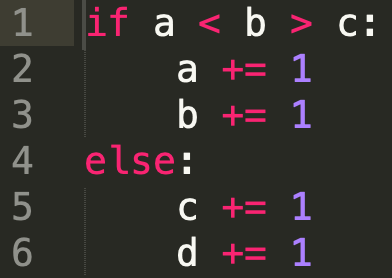
\includegraphics[width=0.33\textwidth]{img/condition1_code.png}}\hfill
\subfloat[Before\label{fig:condition1_before}] {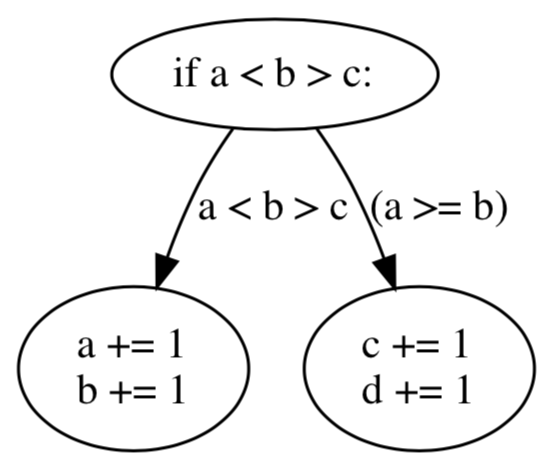
\includegraphics[width=0.33\textwidth]{img/condition1_before.png}}\hfill
\subfloat[After\label{fig:condition1_after}] {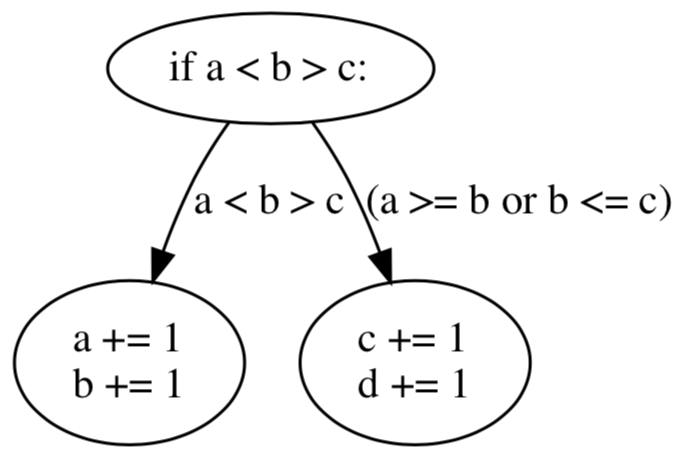
\includegraphics[width=0.33\textwidth]{img/condition1_after.png}}\hfill
\caption{Fixed Logic Inversion Bug} \label{fig:condition1}
\end{figure}

\begin{figure}[H]
\centering
\subfloat[Code\label{fig:condition2_code}]{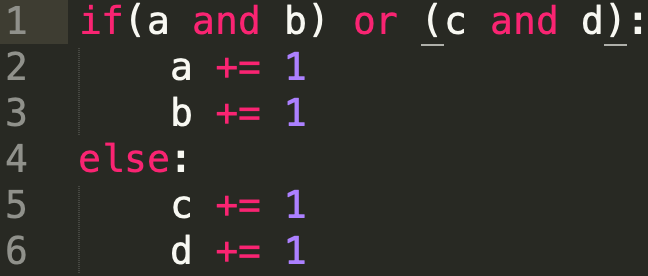
\includegraphics[width=0.33\textwidth]{img/condition2_code.png}}\hfill
\subfloat[Before\label{fig:condition2_before}] {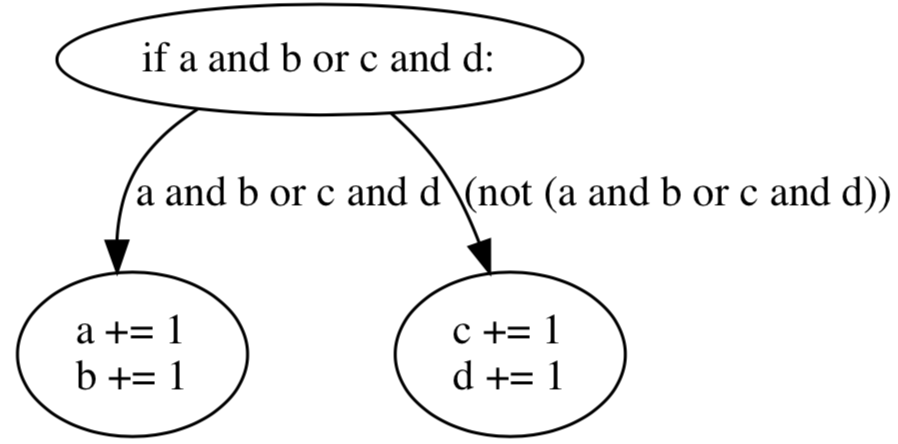
\includegraphics[width=0.33\textwidth]{img/condition2_before.png}}\hfill
\subfloat[After\label{fig:condition2_after}] {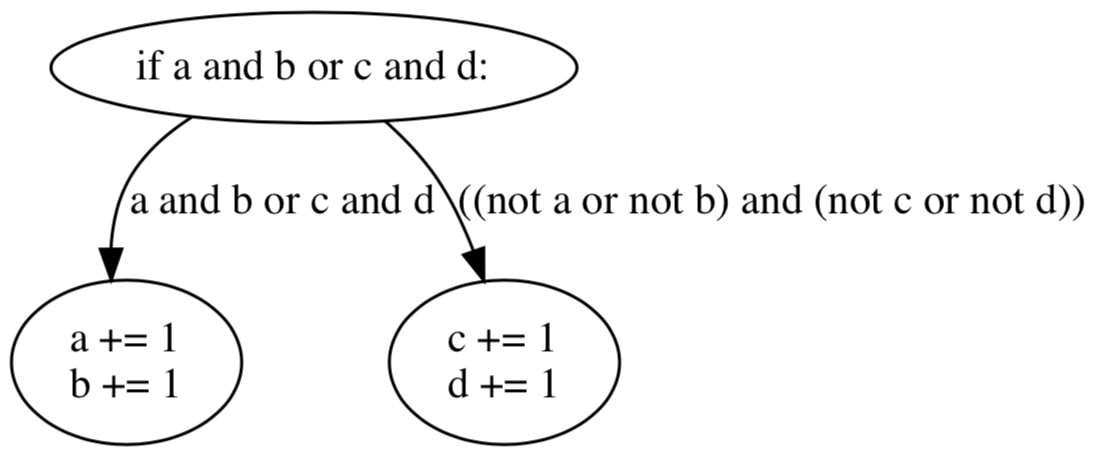
\includegraphics[width=0.33\textwidth]{img/condition2_after.png}}\hfill
\caption{Inversed Logic Using De Morgan's Law} \label{fig:condition2}
\end{figure}

\subsection{For Loop}
\begin{figure}[H]
\centering
\subfloat[Code\label{fig:forelse_code}]{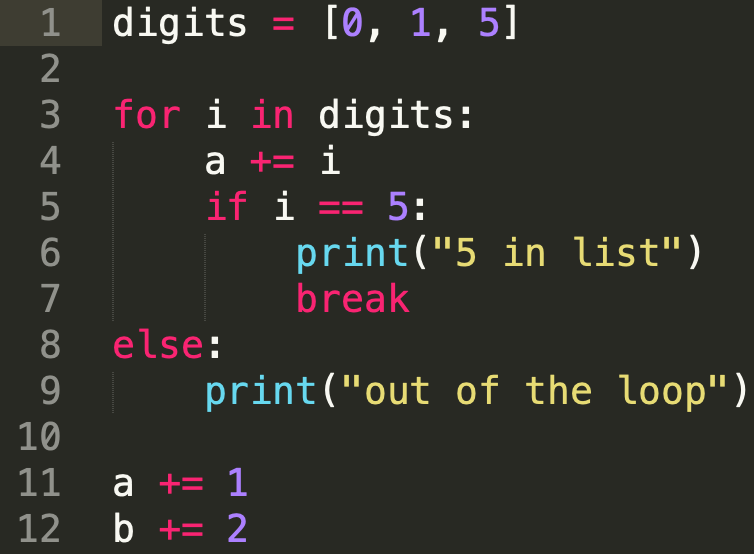
\includegraphics[width=0.30\textwidth]{img/forelse_code.png}}\hfill
\subfloat[Before\label{fig:forelse_before}] {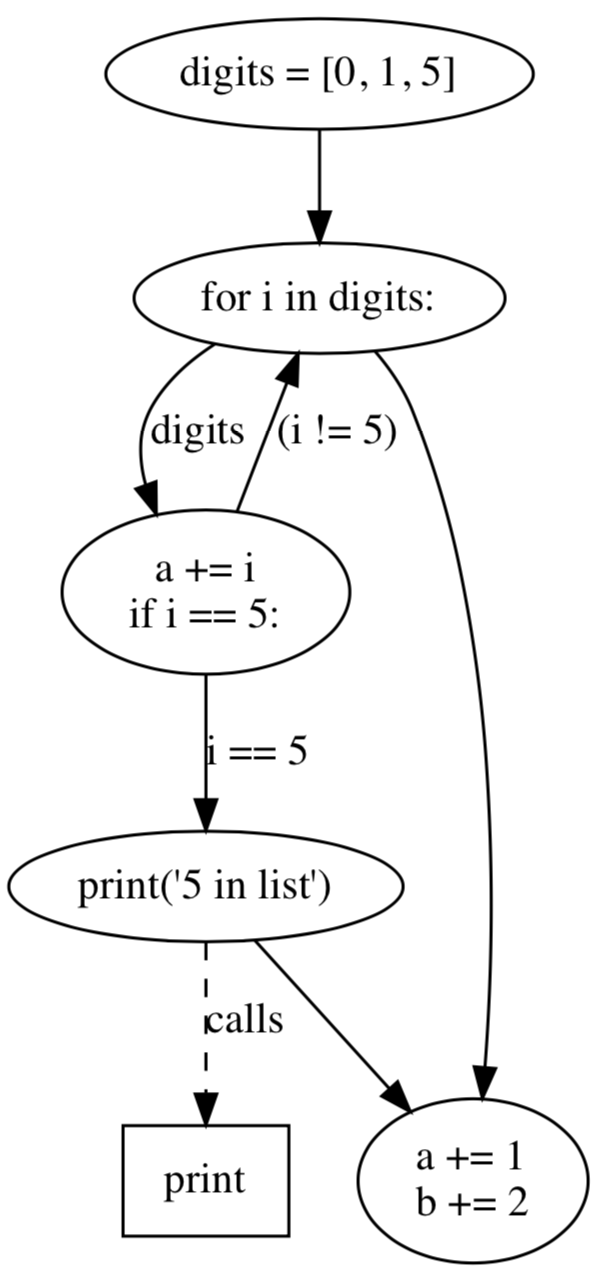
\includegraphics[width=0.22\textwidth]{img/forelse_before.png}}\hfill
\subfloat[After\label{fig:forelse_after}] {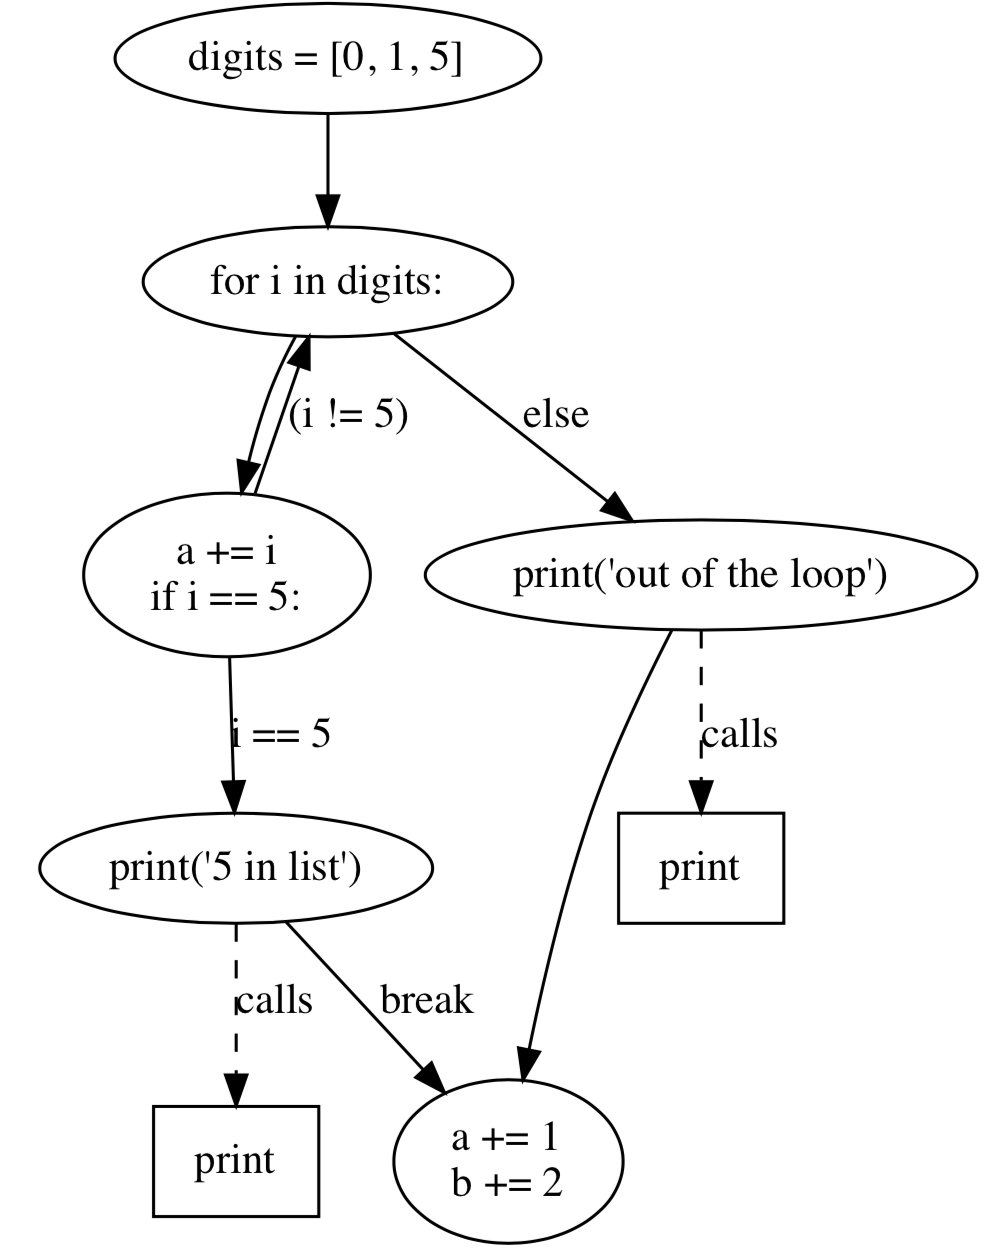
\includegraphics[width=0.37\textwidth]{img/forelse_after.png}}\hfill
\caption{Showed Else part and the Correct Logic in For Loop} \label{fig:forelse}
\end{figure}
\vspace*{-.2cm}
\subsection{While Loop}
\begin{figure}[H]
\centering
\subfloat[Code\label{fig:whileelse_code}]{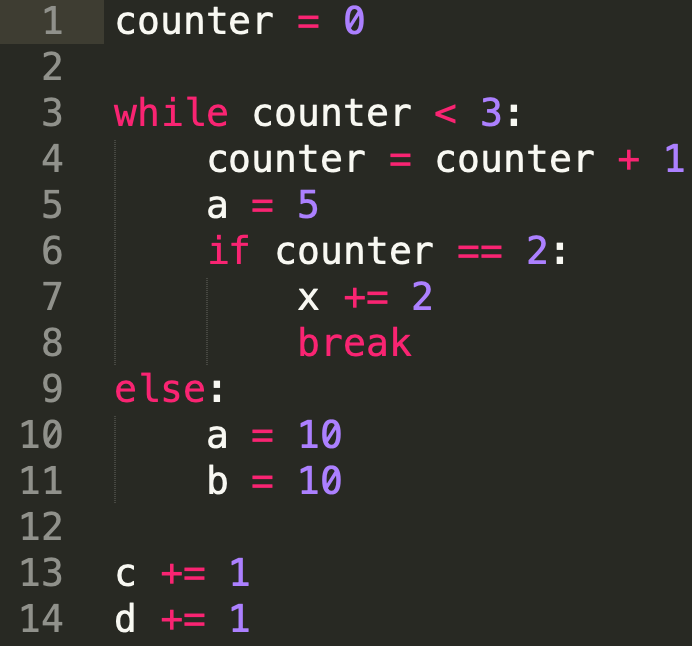
\includegraphics[width=0.30\textwidth]{img/whileelse_code.png}}\hfill
\subfloat[Before\label{fig:whileelse_before}] {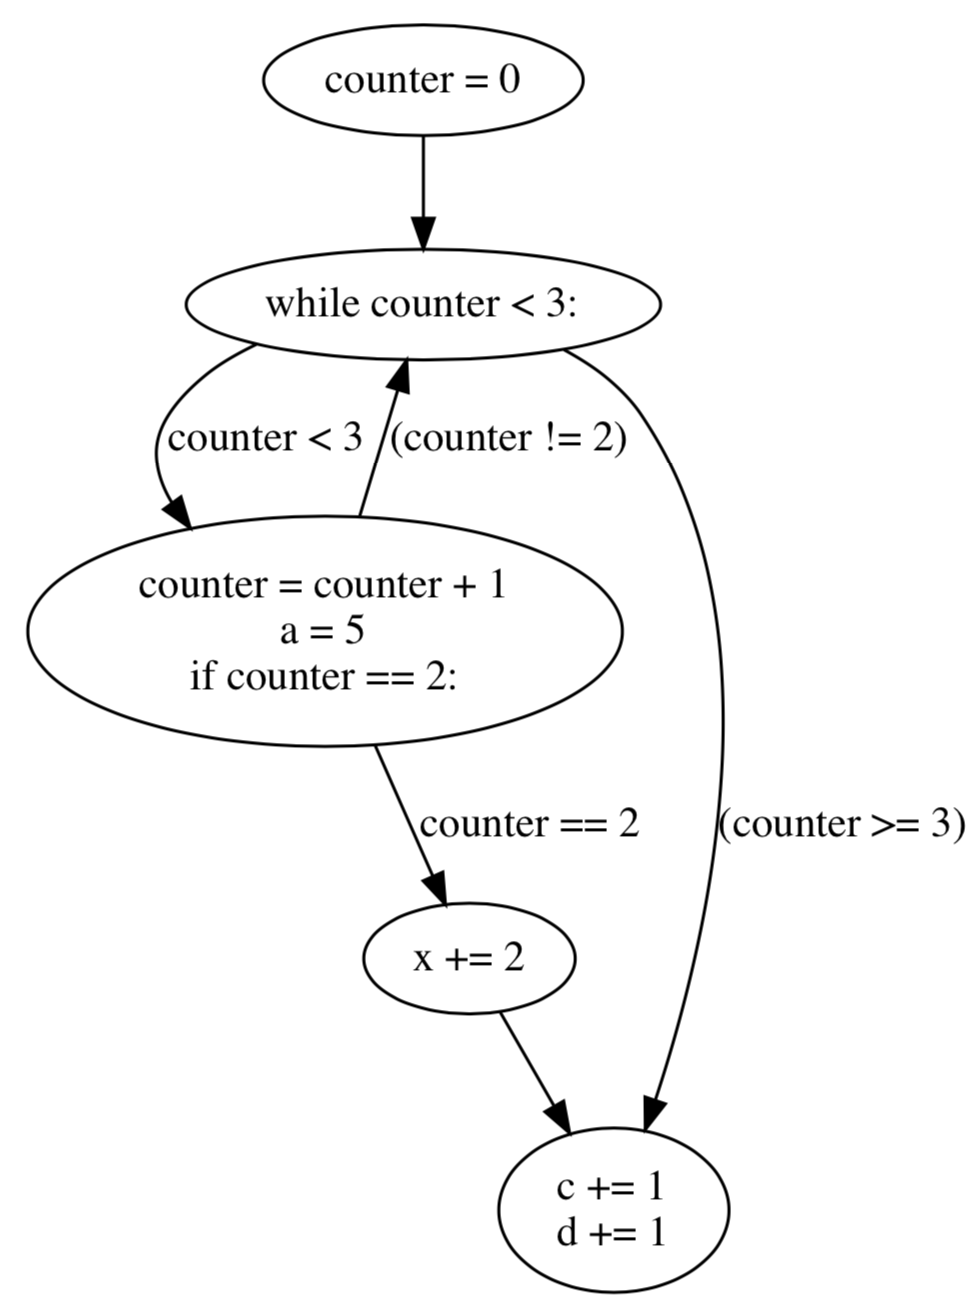
\includegraphics[width=0.35\textwidth]{img/whileelse_before.png}}\hfill
\subfloat[After\label{fig:whileelse_after}] {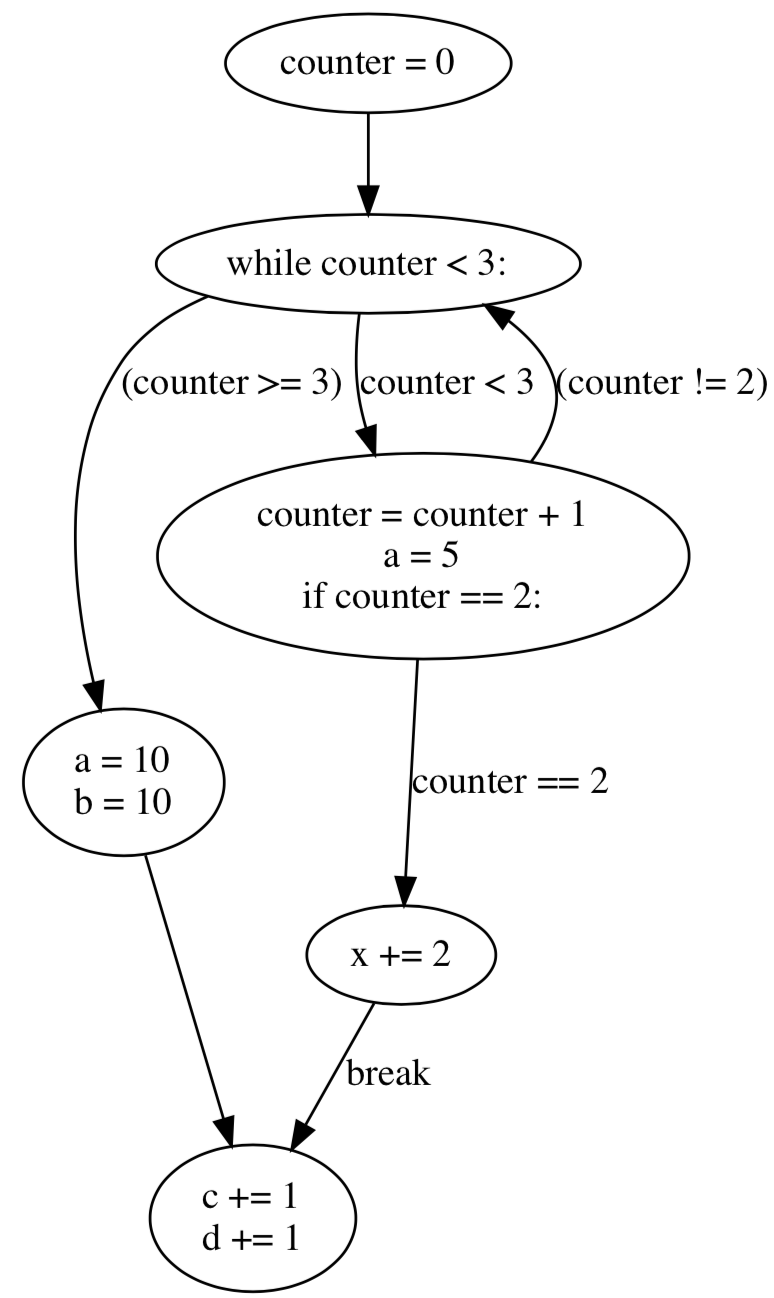
\includegraphics[width=0.28\textwidth]{img/whileelse_after.png}}\hfill
\caption{Showed Else part and the Correct Logic in While Loop} \label{fig:whileelse}
\end{figure}

\subsection{Try}
\begin{figure}[H]
\centering
\subfloat[Code\label{fig:try_code}]{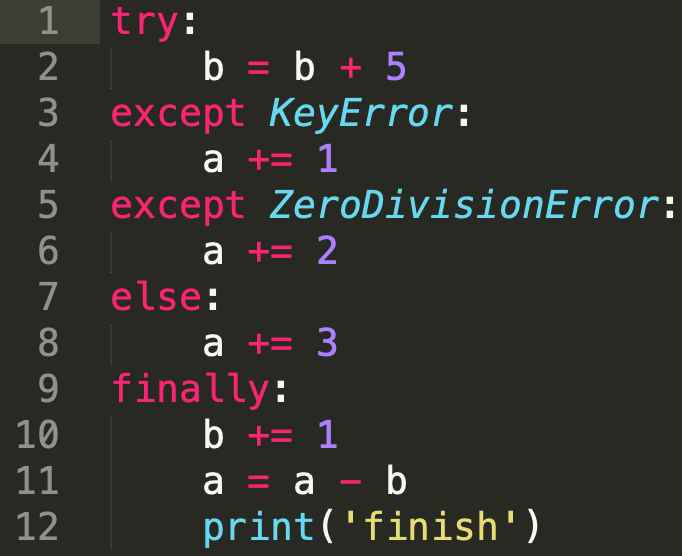
\includegraphics[width=0.28\textwidth]{img/try_code.png}}\hfill
\subfloat[Before\label{fig:try_before}] {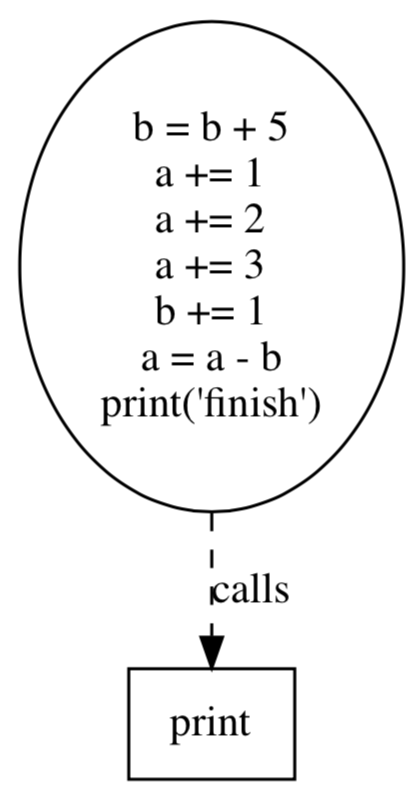
\includegraphics[width=0.18\textwidth]{img/try_before.png}}\hfill
\subfloat[After\label{fig:try_after}] {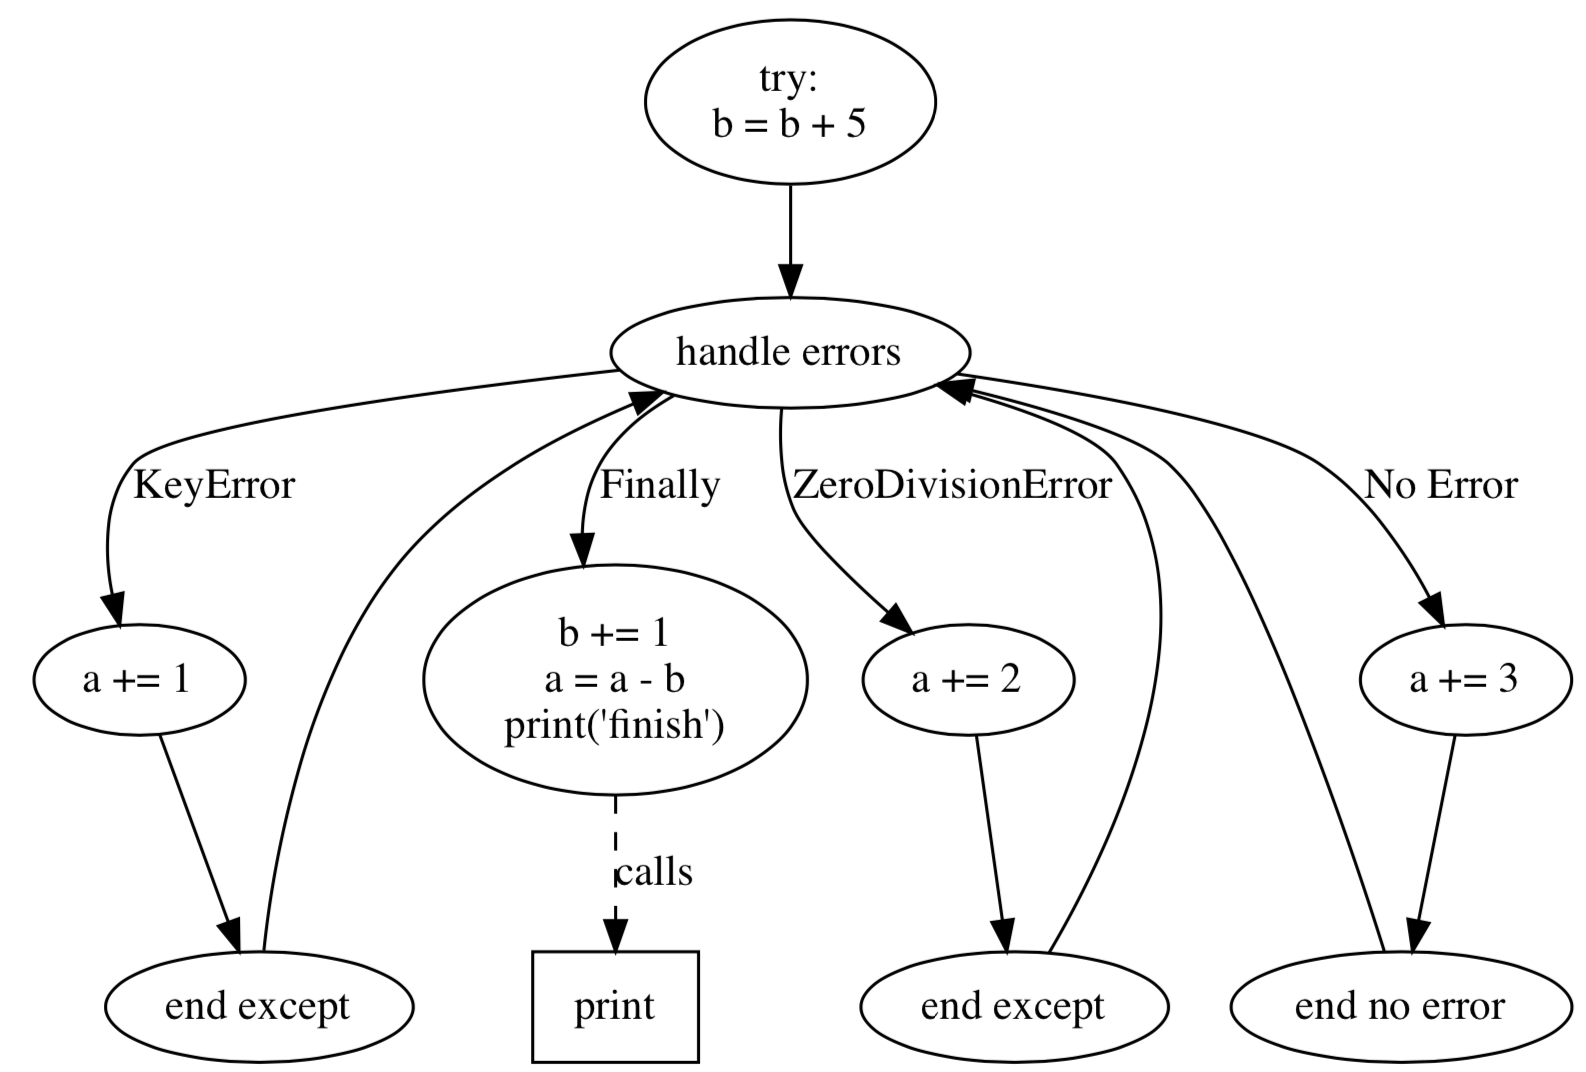
\includegraphics[width=0.52\textwidth]{img/try_after.png}}\hfill
\caption{Added Support for Try} \label{fig:try}
\end{figure}

\subsection{Comprehensions}
The original implementation will show list/dict/set comprehensions directly. For code:
\begin{lstlisting}
a = [2 * x for x in y if x > 0 for y in z if y[0] < 3]
a = {3 * k : 2*v for (k, v) in b.items() if k > 0 if v > 0}
a = {6-x for x in y if x > 5 for y in [1,2,3,4] if y==3}
\end{lstlisting}
The output will be:
\begin{figure}[H]
  \centering
  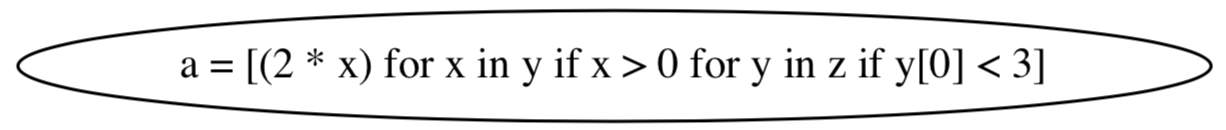
\includegraphics[width=.76\textwidth]{img/listcomp_before.png}
\end{figure}
\vspace*{-.85cm}
\begin{figure}[H]
  \centering
  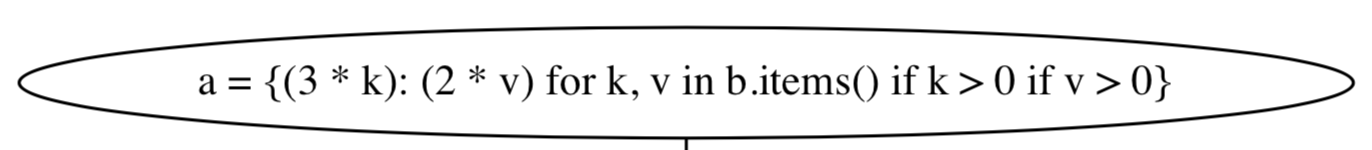
\includegraphics[width=.8\textwidth]{img/dictcomp_before.png}
\end{figure}
\vspace*{-.7cm}
\begin{figure}[H]
  \centering
  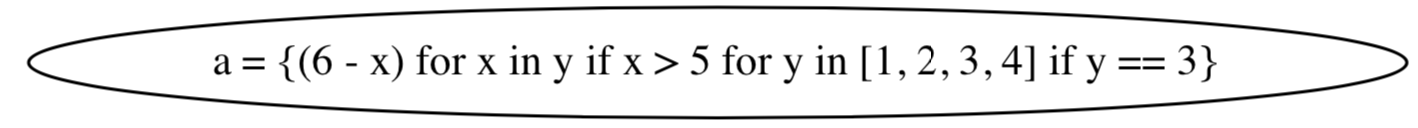
\includegraphics[width=.8\textwidth]{img/setcomp_before.png}
\end{figure}
\noindent
After the implementation, the outputs are:

\begin{figure}[H]
\centering
\subfloat[List Comprehension\label{fig:listcomp_after}]{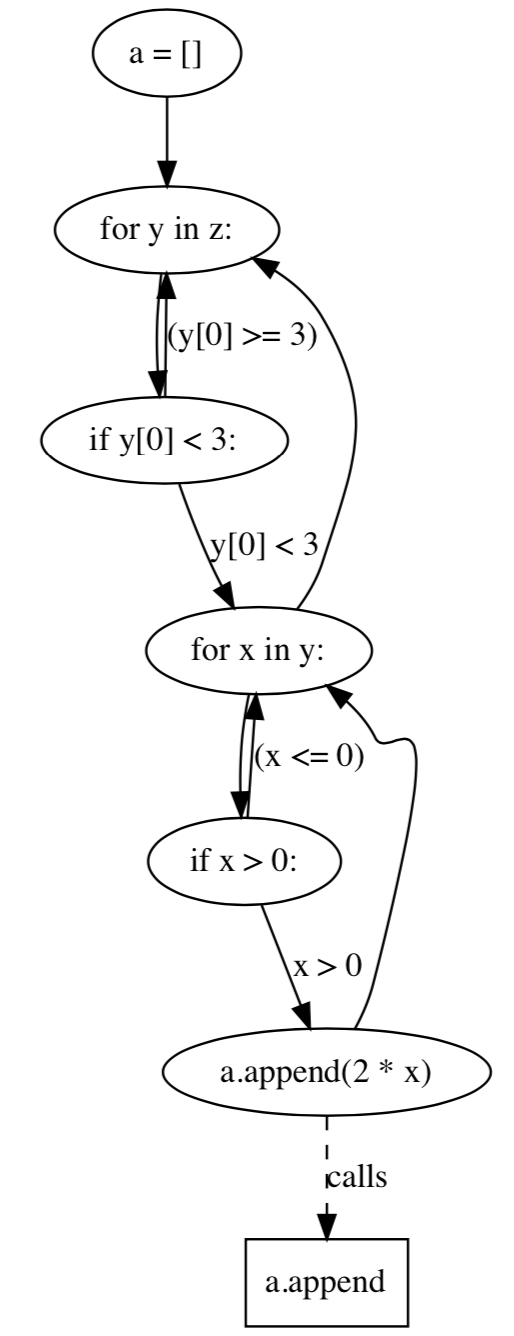
\includegraphics[height=3.5in]{img/listcomp_after.png}}\hfill
\subfloat[Dict Comprehension\label{fig:dictcomp_after}] {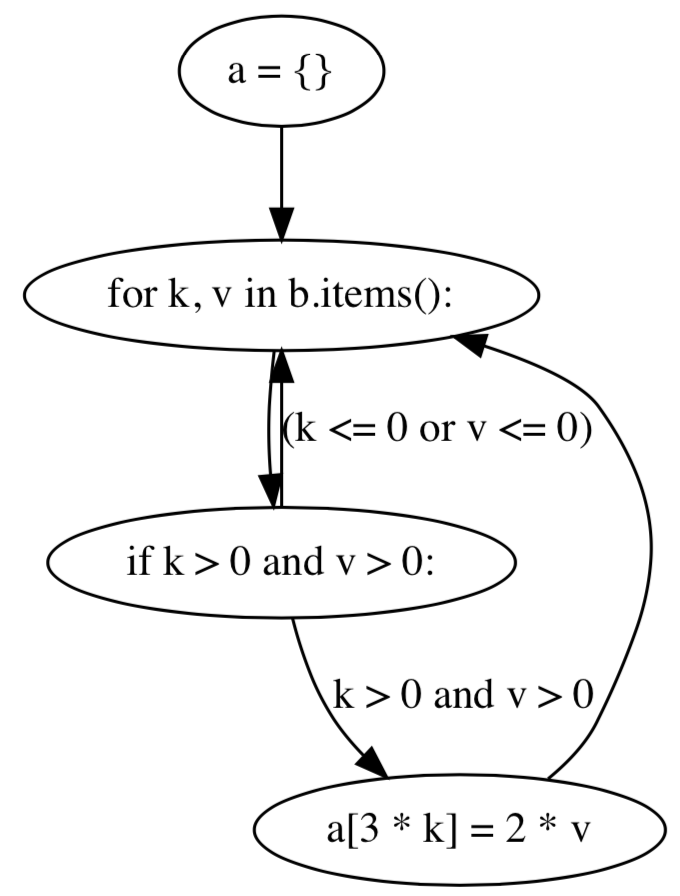
\includegraphics[height=3.5in]{img/dictcomp_after.png}}\hfill
\subfloat[Set Comprehension\label{fig:setcomp_after}] {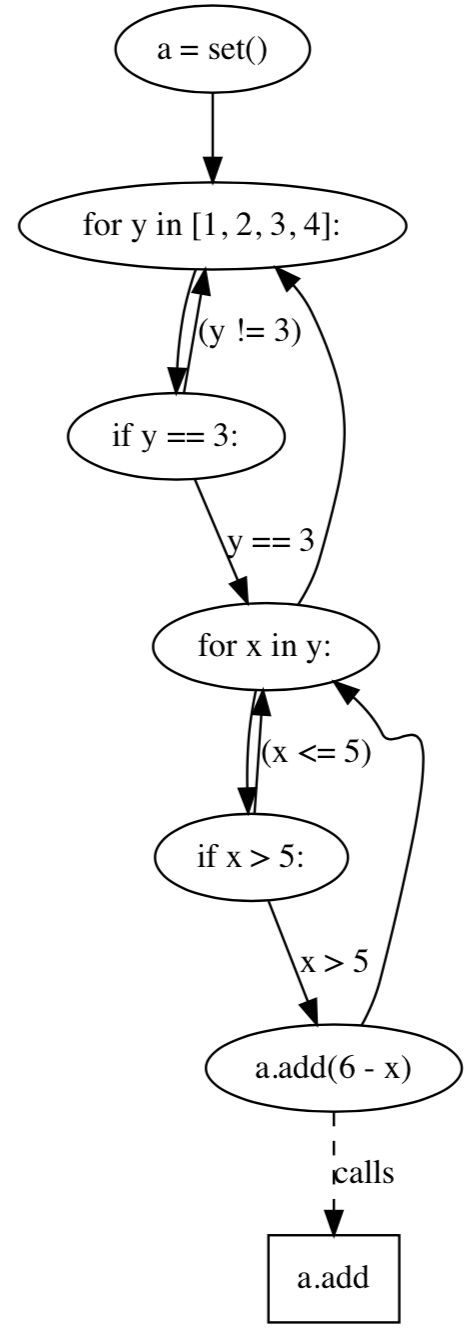
\includegraphics[height=3.5in]{img/setcomp_after.png}}\hfill
\caption{Added Support for Comprehensions} \label{fig:comprehensions}
\end{figure}

\subsection{Lambda Expression and Generator Expression}
The original implementation will show lambda expression and generator expression directly. For code:
\begin{lstlisting}
a = lambda x: 2 * x + 5 if x > 10 else 10 if x == 10 else 3 * x
a = (2*x for x in y if x > 4 for y in [1,2,3,4])
\end{lstlisting}
The output will be:
\begin{figure}[H]
  \centering
  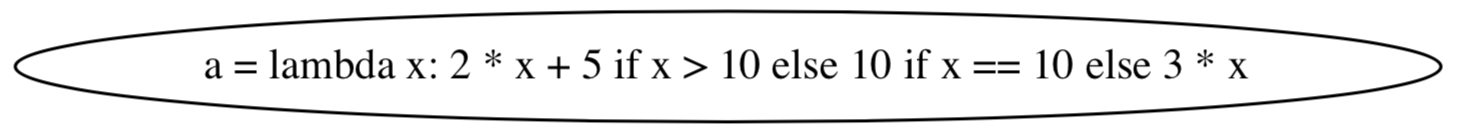
\includegraphics[width=.85\textwidth]{img/lambdaexp_before.png}
\end{figure}
\vspace*{-.8cm}
\begin{figure}[H]
  \centering
  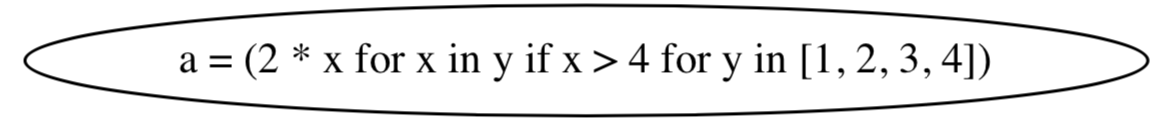
\includegraphics[width=.85\textwidth]{img/genexp_before.png}
\end{figure}
\noindent
After the implementation a separate function is defined. The outputs are:

\begin{figure}[H]
\centering
\subfloat[Lambda Expression\label{fig:lambdaexp_after}]{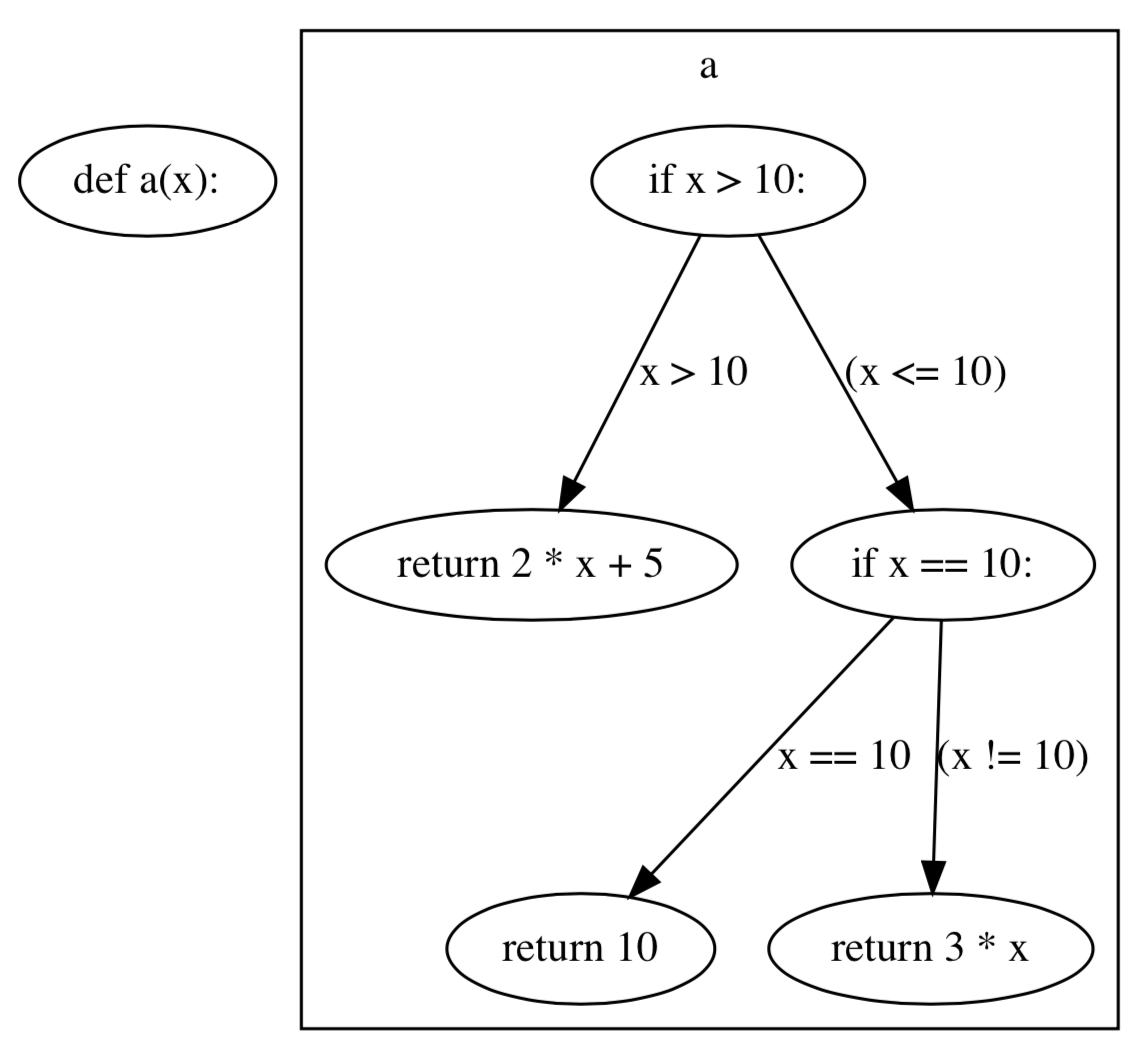
\includegraphics[height=3in]{img/lambdaexp_after.png}}\hfill
\subfloat[Generator Expression\label{fig:genexp_after}] {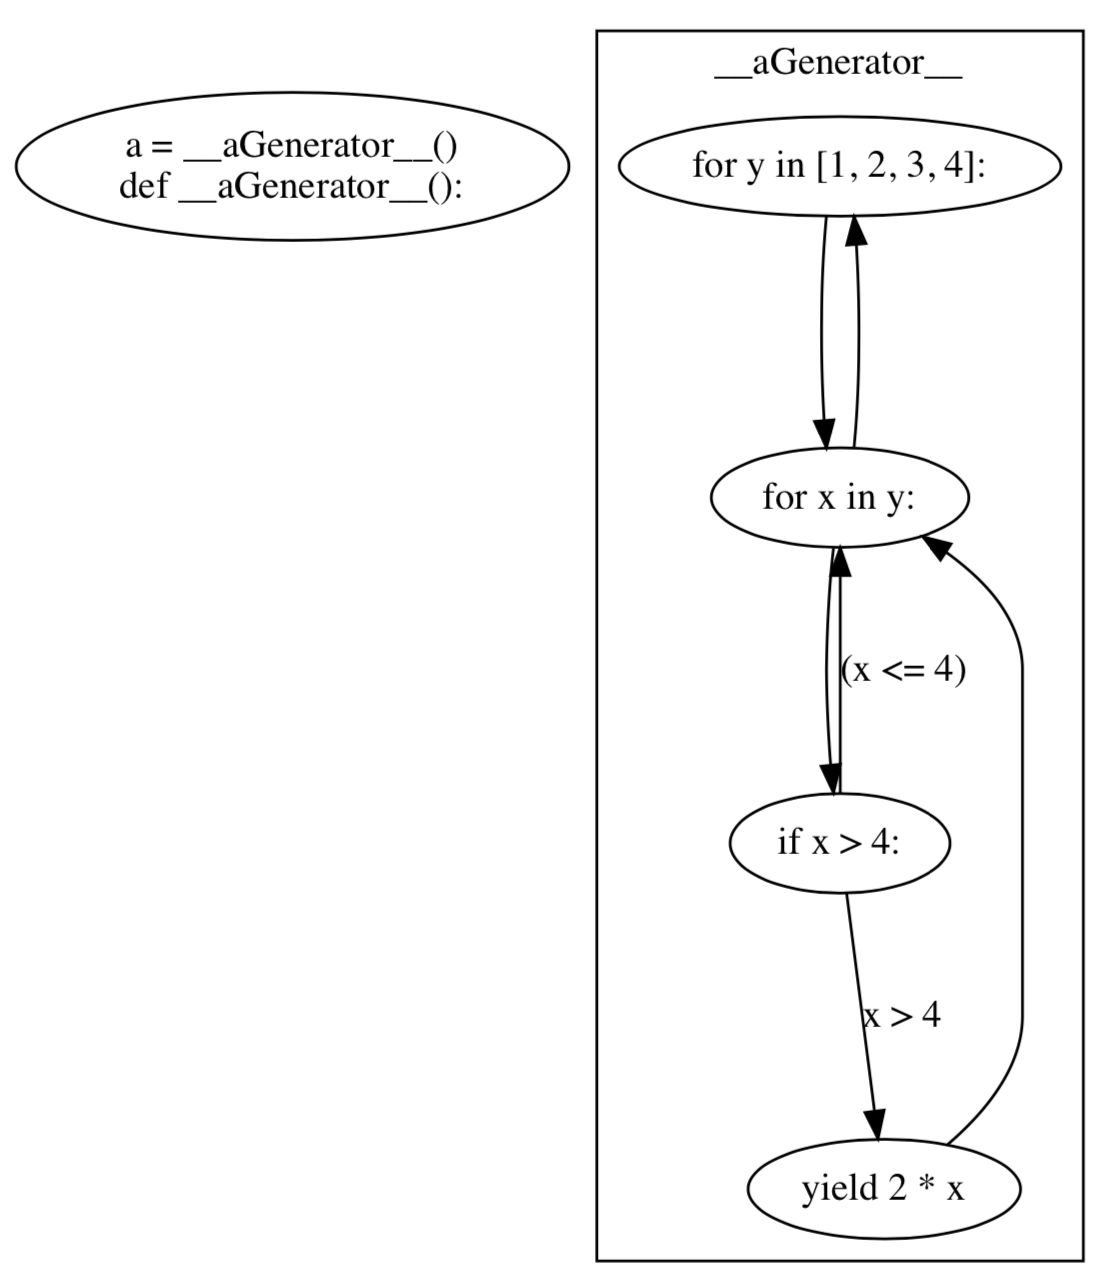
\includegraphics[height=3in]{img/genexp_after.png}}\hfill
\caption{Added Support for Lambda} \label{fig:lambdaexp}
\end{figure}

\section{Conclusion}\label{conclusion}
This report summarized the design and implementation of a control flow graph generator and briefly discussed its testing method. Comparing to other CFG generator, this one focuses on details like the visualization of the lambda function, try catch methods, list/set/dict comprehensions and special usage in While and For loops, etc. It serves as a great supplement for other CFG generators to generate graphs for special cases.
\end{document}




